% Inbuilt themes in beamer
\documentclass{beamer}


%Defining some colours
\definecolor{darkred}{rgb}{0.8,0,0}

% Theme choice: there a number of preset themes to choose from
% Play around with them, Cambridge is nice for first pres
%\usetheme{Szeged}
\usetheme{CambridgeUS} %setting the main theme
%\usecolortheme{beaver} % setting colour theme
\usefonttheme{professionalfonts} %font theme
\useinnertheme[shadow=true]{rounded}
%\useoutertheme{} %outer theme

%\setbeamertemplate{footline} %Remove footer line in all slides
\setbeamertemplate{navigation symbols}{} %removes navigation symbols
\setbeamertemplate{footline}[page number] %removes footer line, keeps pg#
\setbeamertemplate{caption}{\insertcaption} 

%Setting colours for boxes and captions
\setbeamercolor{block title}{bg=darkred, fg=white}
\setbeamercolor{block body}{bg=darkred!10}

% For the Flowchart
\usepackage{tikz}
\usetikzlibrary{shapes.geometric, arrows}
\tikzstyle{startstop} = [rectangle, rounded corners, minimum width=3cm, minimum height=1cm,text centered, draw=black, fill=red!30]
\tikzstyle{process} = [rectangle, minimum width=3cm, minimum height=1cm, text centered, draw=black, fill=orange!30]
\tikzstyle{decision} = [diamond, minimum width=3cm, minimum height=1cm, text centered, draw=black, fill=green!30]
\tikzstyle{arrow} = [thick,->,>=stealth]


% Title page details: 
\title[BEAP Dec 2022]{Creating an Evolution Simulator for Protein Low Complexity Regions and Attempting to Utilize it for an Approximate Bayesian Computation} 
\author{Alexander Turco}
\date{December 5, 2022}
\logo{\includegraphics[height=1cm, width=1cm]{logo.png}}

% Bibliography stuff
\usepackage[natbib=true, sorting=nyt, style=authoryear-comp]{biblatex}
\addbibresource{ABC1.bib}

%Extra packages
\usepackage{makecell}

%For itemize
\setbeamertemplate{itemize item}[triangle]



\begin{document}
	
	% For my introduction slides, there will be the slide with my title and name as well as an outline slide with the brief overview of what I will discuss.
	% Title page frame - SLIDE 1%%%%%%%%%%%%%%%%%%%%%%%%%%%%%%%%%%%%%%%%%%%%%%%%%%%%%%%%%%%%%%%%%%%%%%%%%%%%%%%%%%%%%%%%%%%%%%%%%%%%%%%%%%%%%%%%%%%%%%%%%%%%%%%%%%%%
	\section{Introduction}
	\begin{frame}
		\titlepage 
	\end{frame}
	
	% Remove logo from the next slides
	\logo{}
	
	% Outline frame - SLIDE 2
	\begin{frame}{Overview}
		
		\begin{center}
		\begin{minipage}{6cm}
				
		  		\begin{block}{} \hyperlink{link1}{Background Information} \end{block}
		  		\begin{block}{} Simulating LCR Evolution \end{block}
		  		\begin{block}{} Applications to ABC-MCMC \end{block}
		  		\begin{block}{} Conclusions \end{block}
		  		\begin{block}{} Acknowledgements \end{block}

		\end{minipage}
		\end{center}
	
	\end{frame}
	
	% For my Background slides, I will talk about important things such as WHat LCRs are, their evolution, stuff like that
	% SLIDE 3 - WHAT ARE LCRs%%%%%%%%%%%%%%%%%%%%%%%%%%%%%%%%%%%%%%%%%%%%%%%%%%%%%%%%%%%%%%%%%%%%%%%%%%%%%%%%%%%%%%%%%%%%%%%%%%%%%%%%%%%%%%%%%%%%%%%%%%%%%%%%%%%%%%
	% The graphic for this slide is an image of some output from segA with the parameters in the brackets
	\section{Background}
	\begin{frame}{What are Low Complexity Regions?}
		\label{link1}
		
		\begin{block}{\textit{Saccharomyces cerevisiae} SRP40 Protein LCRs}
			$>$CAA82171.1(25-125) complexity=0.92 (15/1.90/2.20)
			sssssssssssssssssssssssssgessssssssssssssdssdssdsessssssssss
			ssssssdsesssesdssssgsssssssssdesssesesede \newline
			
			$>$CAA82171.1(149-282) complexity=1.33 (15/1.90/2.20)
			esssssessssgsssssesesgsesdsdsssssssssdsesdsesdsqssssssssdsss
			dsdssssdsssdsdssssssssssdsdsdsdsssdsdssgssdsssssdsssdestssds
			sdsdsdsdsgssse \newline
			
			$>$CAA82171.1(298-316) complexity=2.18 (15/1.90/2.20)
			tpassnestpsasssssan
			
		\end{block}		
		
	\end{frame}

	% SLIDE 4 - I do Not Know if I am including this slide
	% The Graphic for this slide is an  
	% Entropy, which is measured by Shannon's Entropy equation is a measure of compositional complexity which uses the proportion of residue(s)
	% in a subsequence to measure the compositional state of that subseequence - A lower variety of residues = lower entropy 
	%\begin{frame}{Shannon's Entropy - MAYBE }
		
	%		$H = -L\sum p_i log_2(p_i)$
		
	%\end{frame}

	%SLIDE 5 - LCR's PRESENT IN UNIQUE WAYS
	\begin{frame}{LCRs Present in Unique Ways }
		
		\begin{alertblock}{Homorepeats}
			Consecutive iterations of a single residue
		\end{alertblock}
	
		\begin{center}
			\includegraphics[width=5cm, height=1cm]{poyglut.png}
		\end{center}
	
		\begin{alertblock}{Direpeats}
			Consecutive iterations of two ordered, different residues
		\end{alertblock}
	
		\begin{center}
			\includegraphics[width=5cm, height=1cm]{direpeat.png}
		\end{center}

		\begin{alertblock}{Imperfect Repeats}
			Regions in which the repeat units are not the same
		\end{alertblock}
	
		\begin{center}
			\includegraphics[width=6cm, height=1.2cm]{imperfect.png}
		\end{center}
	
	\end{frame}

	%SLIDE 6 LCRs are hypermutable
	% Maybe change the lines from the fly to dashed - as per photo Lauren Sent
	\begin{frame}{LCRs are Hypermutable }
		
		
		\begin{center}	
		\includegraphics[width=8cm, height=3cm]{drosophila.png}
		\end{center}
	
		\begin{center}	
		\begin{tabular}{|cccc|}
			\hline
			\makecell{\textbf{mam} \\ \textbf{domain}} & \textbf{Size (bp)} & \makecell{\textbf{Amino Acid} \\ \textbf{Substitutions}} & \makecell{\textbf{Amino Acid/} \\ \textbf{Total Substitutions}}  \\ 
			\hline
			Unique & 933 & 26 & 0.15\\ 
			\hline
			Repetitive & 810 & 47 & 0.42\\ 
			\hline
		\end{tabular}\newline\newline
		\end{center}
	
	%\footer{\tiny\citep{newfeld1991interspecific}}
	\footnotetext[1]{\tiny\cite{newfeld1991interspecific}}	
	\end{frame}

	%SLIDE 7 - Mechanisms of LCR Evolution
	\begin{frame}{Proposed Mechanisms of LCR Evolution}
		\textit{1. Polymerase Slippage/Slipped Strand Mispairing}
		\begin{columns}
			
			\column{0.5\textwidth}
			\centering
			\begin{figure}
				\includegraphics[width=\columnwidth, height=2.5cm]{slippage2n.png} \\~\\
				\caption{\centering \textbf{Polymerase Slips Forward}}
			\end{figure}
			
			\column{0.5\textwidth}
			\centering
			\begin{figure}
				\vspace{0.5cm}
				\includegraphics[width=\columnwidth, height=2.5cm]{slippage1n.png} \\~\\
				\caption{\centering \textbf{Polymerase Slips Backwards}}
			\end{figure}
		
		\end{columns}
	
	\footnotetext[2]{\tiny\cite{levinson1987slipped,sehn2015insertions}}
	\end{frame}

	%SLIDE 8 - Mechanisms of LCR Evolution
	\begin{frame}{Proposed Mechanisms of LCR Evolution}
		\textit{2. Unequal Recombination} \newline\newline
		
		\begin{figure}
			\includegraphics[width=8cm, height=1.8cm]{unequal.png} \\~\\
		\end{figure}
		
	\footnotetext[3]{\tiny\cite{mirkin2007expandable}}	
	\end{frame}
	
	%SLIDE 8 - Why Care About LCR Evolution?
	\begin{frame}{Why Care about LCRs and their Evolution?}
	
	\begin{center}	
		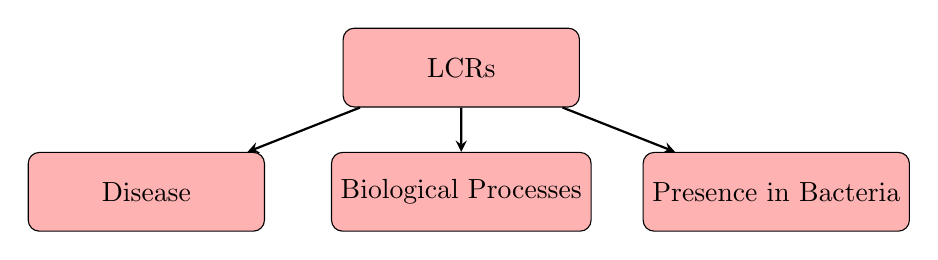
\begin{tikzpicture}[node distance=2cm]
			\node[startstop] (1) {Disease};
			\node[startstop, right of=1, xshift=2cm] (2) {Biological Processes};
			\node[startstop, right of=2, xshift=2cm] (3) {Presence in Bacteria};
			\node[startstop, above=2, xshift=4cm, yshift=1cm] (4) {LCRs};
			
			\draw [arrow] (4) -- (1);
			\draw [arrow] (4) -- (2);
			\draw [arrow] (4) -- (3);
			
		\end{tikzpicture}
	\end{center}

		\begin{columns}
			
			\column{0.33\textwidth}
			\centering
			\begin{figure}
				\includegraphics[width=\columnwidth, height=2.5cm]{huntington.jpg} \\~\\
				\caption{\centering \textit{Huntington's Disease}}
			\end{figure}
			
			\column{0.33\textwidth}
			\centering
			\begin{figure}
				\includegraphics[width=2.5cm, height=2.5cm]{chrom.png} \\~\\
				\caption{\centering \textit{Genetic Recombination}}
			\end{figure}
		
			\column{0.33\textwidth}
			\centering
			\begin{figure}
				\vspace{-0.4cm}
				\includegraphics[width=\columnwidth, height=2.5cm]{menin.jpg} \\~\\
				\caption{\centering \textit{Neisseria meningitidis}}
			\end{figure}
			
		\end{columns}
	
	\end{frame}

	\begin{frame}{What we Did in this Study}
		\begin{itemize}
			\item Utilized \texttt{C++} to build an evolution simulator which altered protein sequences via point mutations, insertions, and deletions \newline
			\item Tested the simulator with various insertion/deletion rates and mutation rates \newline
			\item Attempted to program an ABC-MCMC in \texttt{C++} using the evolution simulator as an important step in the algorithm, in order to estimate parameters like mutation and indel rates.
		\end{itemize}
	\end{frame}

	%For my Research questions/Exploration slides, I will talk about things such as
	%SLIDE 9%%%%%%%%%%%%%%%%%%%%%%%%%%%%%%%%%%%%%%%%%%%%%%%%%%%%%%%%%%%%%%%%%%%%%%%%%%%%%%%%%%%%%%%%%%%%%%%%%%%%%%%%%%%%%%%%%%%%%%%%%%%%%%%%%%%%%%%%%%%%%%%%
	\section{Simulating LCR Evolution}
	
	\begin{frame}{LCR Simulator Overall Process}
		\begin{center}
			\begin{enumerate}
			\item mutation rate = 0.14
				indel rate = 0.14 \newline
				Random Protein Sequence \newline	
				GGAGGGAQ \newline\pause	
				
				\item Assign Exponential Deviates \newline
				mutation deviates = (0.83, 1.82, 2.35, 0.54, 0.98, 0.76, 1.53, 2.34) \newline
				indel deviates = (0.21, 1.21, 1.49, 0.86, 0.97, 1.13, 0.53, 0.35) \newline
				\qquad exp($\beta$), where $\beta$ = mutation rate\newline 
				\qquad exp($\beta$), where $\beta$ = length of repeat * indel rate \newline \pause
				
				\item Point Mutation, Insertion, or Deletion \newline
				Lowest value deviate = Residue that mutates fastest \newline \pause
				
				\item Upon point mutation, insertion, or deletion, scan the sequence again to see if the landscape of the sequence was affected, assign new deviates to affected amino acids only.
				
			\end{enumerate}
		\end{center}	
	\end{frame}

	\begin{frame}{LCR Simulator Results}
		\includegraphics[height=6cm, width=\textwidth]{im0.01-0.1-0.5.jpeg}
	\end{frame}

	\begin{frame}{LCR Simulator Results 2}
		\includegraphics[height=7cm, width=\textwidth]{im1-2-10.jpeg}
	\end{frame}

	\begin{frame}{LCR Simulator Results 3}
		\includegraphics[height=7cm, width=\textwidth]{m0.01-0.1-0.5.jpeg}
	\end{frame}

	\begin{frame}{LCR Simulator Results 4}
		\includegraphics[height=7cm, width=\textwidth]{m1-2-10.jpeg}
	\end{frame}
	
	%Say something like, before we get into how this simulation can be used in an approximate bayesian computation, were just going to go through a very simple overview of bayesian statistics
	\section{Applications to ABC-MCMC}
	\begin{frame}{Bayesian Statistics Overview}
	
	\textbf{Bayesian Statistics: Model-based statistical inference}
	
	\begin{figure}
		
		\begin{equation} \tag{1}
			p(D|\theta)
		\end{equation}
	\caption{\textit{Likelihood}} \pause
	
		\begin{equation} \tag{2}
			p(\theta|D)
		\end{equation}
	\caption{\textit{Posterior}}
	
	\end{figure}
	
	\end{frame}

	%SLIDE 11
	\begin{frame}{Why use an ABC-MCMC}
	
	\uncover<1>{
	\begin{itemize}
		\item The increasing complexity and magnitude of available data can make the likelihood difficult to calculate   \newline
	\end{itemize}
	
	\begin{figure}
	\scalebox{2}{
		$ p(D|\theta)$}
	\end{figure}} \pause
	
	\uncover<2>{
	\begin{figure}
		\vspace{-1.5cm}
		\scalebox{2}{
			$ p(D|\theta)$}
	\end{figure}
		
	\begin{tikzpicture}[remember picture,overlay]
		\node at (current page.center) {\includegraphics[width=5cm]{no.png}};
	\end{tikzpicture}
	
	\begin{figure}
		\vspace{1.5cm}
	\begin{itemize}
		\item Calculation of the likelihood is replaced with a simulation step
	\end{itemize}
	\end{figure}}
	
	\end{frame}

	%Slide 12 - Here put the ABC-MCMC algorithm described by Marjoram (one Brian used in his MCMC slides)
	%%% SO HERE WE NEED TO RE-EVALUATE THE SLIDES - March 18 2023
	\begin{frame}{MCMC for ABC}
		
		\begin{enumerate}
			\item Propose a move from $\theta$ to $\theta'$ according to a transition kernel $q(\theta,\theta')$.
			\item Generate simulated dataset $D'$ using $\theta'$ and calculate $S'$.
			\item If $\rho(S', S) \le \epsilon$ continue to 4, otherwise remain at $\theta$ and go to 1.
			\item Calculate \newline \begin{center}$\alpha(\theta, \theta') = min(1, \frac{\pi(\theta')q(\theta',\theta)}{\pi(\theta)q(\theta, \theta')})$ \end{center}
			\item Accept $\theta'$ with probability $\alpha$, otherwise stay at $\theta$.
			\item Return to 1.
		\end{enumerate}
	
		\footnotetext[4]{\tiny\cite{marjoram2003markov}}	
	\end{frame}

	%Slide 13 - Here we put MY version of the algorithm - We could also put these on the same slide and just compare! SLIDE 14 AND 15
	%Should I put the equation for calculating distance in this slide? or at the end in the appendix idk yet.
	\begin{frame}{MCMC for ABC: Modified Algorithm}
	
		\begin{enumerate}
			\item Propose a move from $\theta$ to $\theta'$ according to the normal distribution $N(0.0,1.0)$
			\item Create and mutate a random protein sequence using $\theta'$ to generate the simulated Dataset $D'$ - do this 1000 times per newly proposed parameter value.
			\item Calculate summary statistics for simulated dataset $D'$ (average of all 1000 vectors of summary statistics)
			\item If $d(S',S) < previous\_distance$, go to next step, otherwise employ a one-sample t-test to assess the probability of accepting a larger distance. If the newly proposed distance is close to the previous distance, there is a higher chance we accept the value, otherwise we reject.
			\item Accept $\theta'$ 
			\item Return to step 1
		\end{enumerate}
	
	\end{frame}

	\begin{frame}{ABC MCMC Preliminary Results}
		\includegraphics[height=6cm, width=\textwidth]{distances.jpeg}
	\end{frame}

	\section{Conclusion}
	\begin{frame}{Conclusions}
		\begin{itemize}
			\item Created and tested a program to simulate the evolution of low complexity regions based off of two evolutionary parameters, mutation and indel rates \newline
			\item The simulation program is compatible in a program written for an ABC-MCMC \newline
			\item Struggling with creating posterior distribution, potentially due to selection of poor summary statistics or a lack of weight placed on each statistic
		\end{itemize}
	\end{frame}

	%\section{Future Work}
	%\begin{frame}{Future Work}
		
		%\begin{itemize}
			%\item Graphical representations of simulation iteration versus parameter values 
		%	\item Implementation of weighted summary statistics in distance calculation
		%	\item Adjustment of values such as mean and standard deviation of the proposal distribution
			
		%	\centering\includegraphics[width=7cm, height=5cm]{graph.png}
			
	%	\end{itemize}
		
	%\end{frame}

	\section{Acknowledgements}
	\begin{frame}{Acknowledgements}
		\begin{itemize}
			\item Dr. Brian Golding \newline
			\item Sam Long \newline
			\item Zachery Dickson \newline
			\item Johanna Enright
		\end{itemize}
	\end{frame}
		
	% Blocks frame
	%\section{Blocks in Beamer}
	%\begin{frame}{Blocks in Beamer}
	%	\begin{block}{Standard Block}
	%		This is a standard block.
	%	\end{block}
	%	\begin{alertblock}{Alert Message}
	%		This block presents alert message.
	%	\end{alertblock}
	%	\begin{exampleblock}{An example of typesetting tool}
	%	\end{exampleblock}
	%\end{frame} 
	
\end{document}
